\section{Implementation}
\subsection{Step Detection}
To determine whether a step is taken, the approach taken by \citet{zhao:pedometer} is implemented. Our implementation first calculates a threshold, which corresponds to the threshold line in \Cref{fig:zhaoGraph}. The threshold is calculated by subtracting the minimum accelerometer measurement from maximum measurement, from the array where the measurements are stored.\\

According to \citet[p. 2]{zhao:pedometer} a step has occurred if there is a negative slope in the acceleration graph and the acceleration curve crosses the threshold. It is determined whether a negative slope has occurred, by comparing the latest accelerometer measurement with the previous one. If the last measurement was above the threshold, and the current is below the threshold, a negative slope which crossed the threshold and thus, a step has occurred.\\

As \citet[p. 2]{zhao:pedometer} we assume that a person can either run as fast as five steps per second or walk as slowly as one step every two seconds. This is handled in the implementation by checking the time since the last measurement. If less than 200 milliseconds have passed since the last step, a new step is not detected. If more than 2 seconds have passed the accelerometer measurement array is updated with a 0 to indicated that the person is not moving.\\

Our implementation utilises an sensitivity threshold so measurements which are very close to each other are not detected as a new step, even though they fulfill the requirements mentioned earlier. This is done to filter out small deviations in measurements which might falsely be identified as a new step.
\begin{figure}[h!]
  \centering
    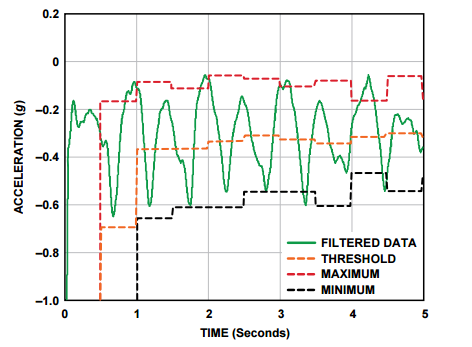
\includegraphics[scale=0.8]{Images/accPlot.png}
  \caption{A acceleration plot from \citet[p. 2]{zhao:pedometer} showing filtered data from a pedometer worn by a person walking}
  \label{fig:zhaoGraph}
\end{figure}
\subsection{Calculation of Steps Per Minute}